马氏规则由俄罗斯化学家马尔科夫尼科夫(Vladimir V.Markovnikov)在1869年提出,而2019年是马氏规则被提出的第150周年。马尔科夫尼科夫是俄罗斯著名科学家布特列洛夫(Alexander Butlerov)的博士生。在他1869年发布的博士论文中,马尔科夫尼科夫提出了几乎每本现今有机化学教科书中都有引用的马氏规则,其指出:当不对称的烯烃或炔烃与卤化氢(包括氯化氢、溴化氢及碘化氢)发生加成反应时,卤化氢中的氢原子加在含氢较多的碳原子上。但是在某些情况中,由于底物和试剂的不同,与上述结论相反的实验结果也被观察到,这种相反的结果被称作反马氏加成。虽然马氏规则是针对卤化氢对烯烃和炔烃的加成反应而提出的,但随着有机化学的发展,许多其它的加成反应因选择性相似而也被相应描述为马氏或反马氏规则。

事实上,马氏规则应该被修改为:对碳碳双键和三键的加成选择性来自于更加稳定的中间体的形成。在某些情况下,除了电子效应之外,空间效应也会影响马氏或反马氏加成产物的比例。

以下问题主要与著名化学家布特列洛夫和他在喀山大学的同事及学生们的各类研究发现有关。

\noindent\textbf{4.1.}
画出下列反应主要产物\textbf{A}-\textbf{E}的结构,注意立体化学(不考虑光学异构)。

\begin{figure}[h]
	\centering
	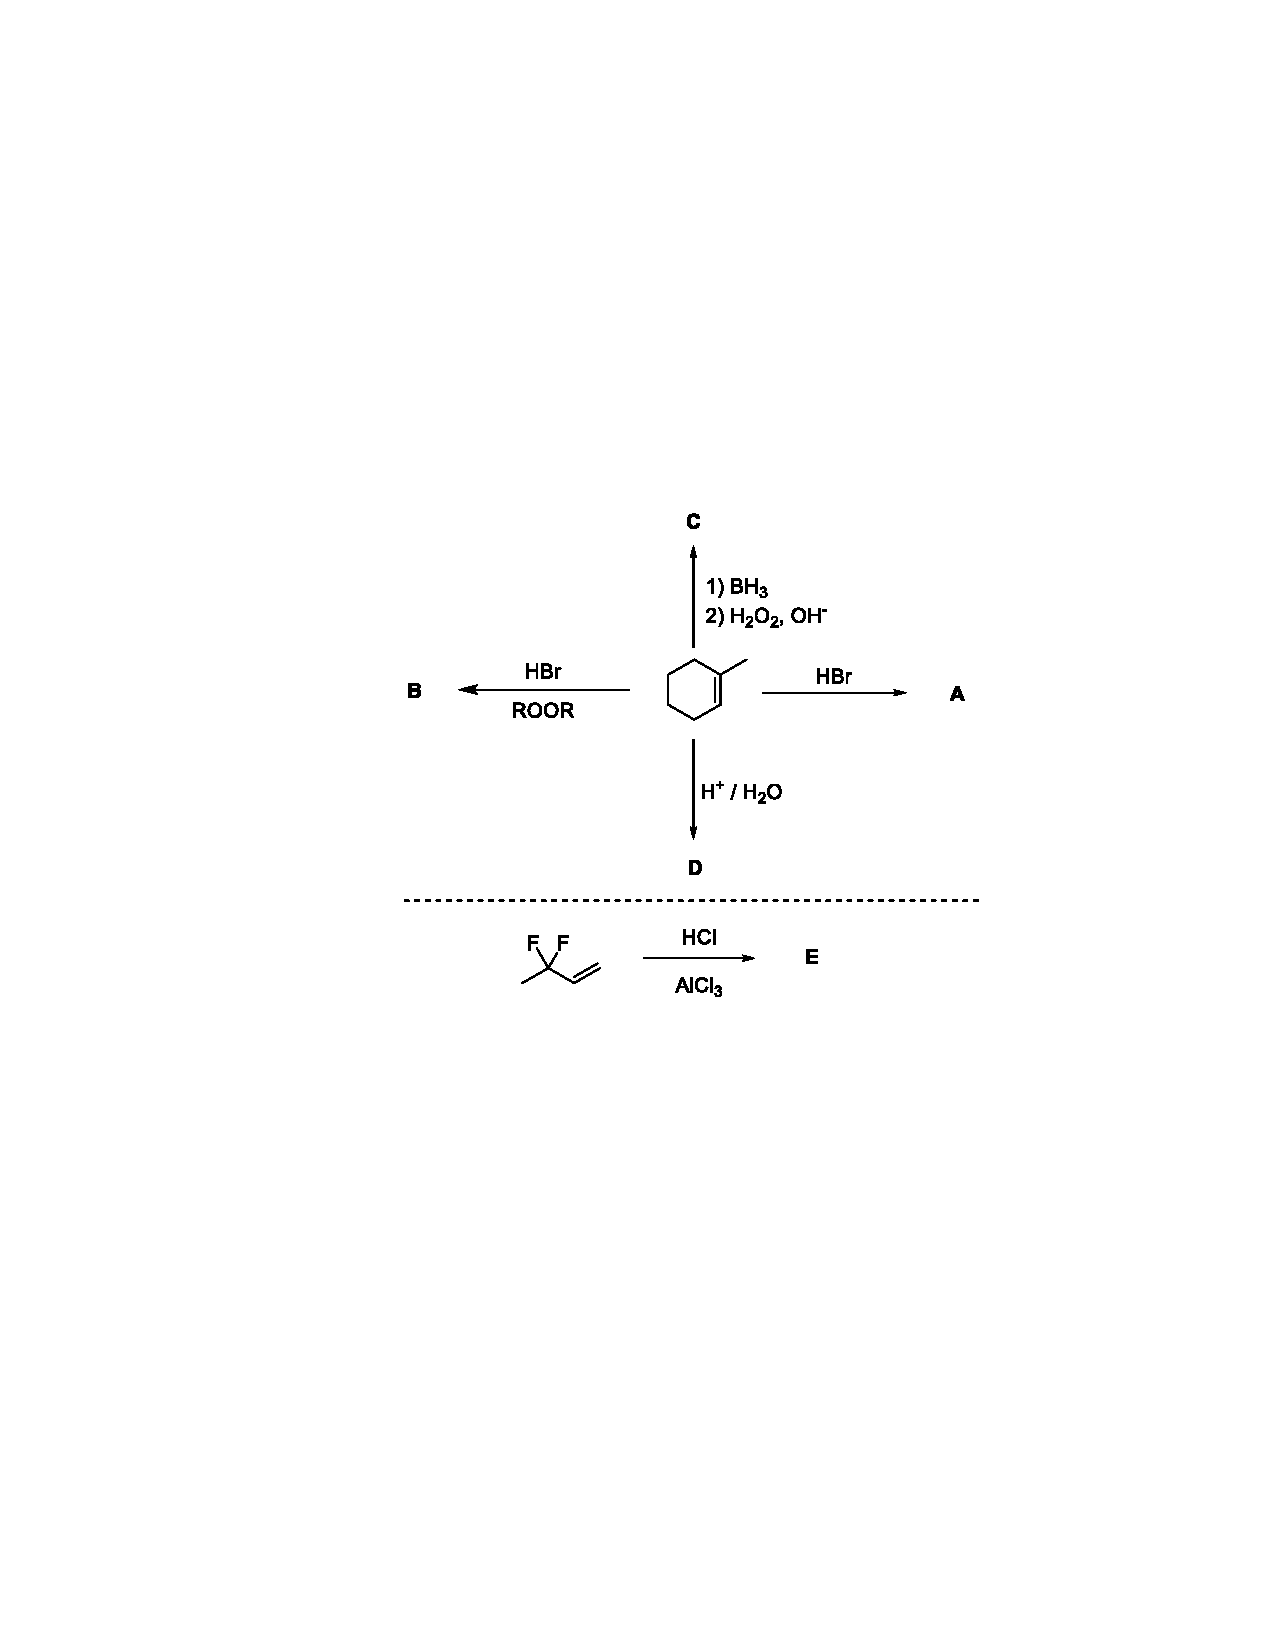
\includegraphics[width=10cm]{./pic/t4-2.pdf}
\end{figure}

\noindent\textbf{4.2.} 画出下列反应的主要产物\textbf{F}和\textbf{G}的结构。

\begin{figure}[h]
	\centering
	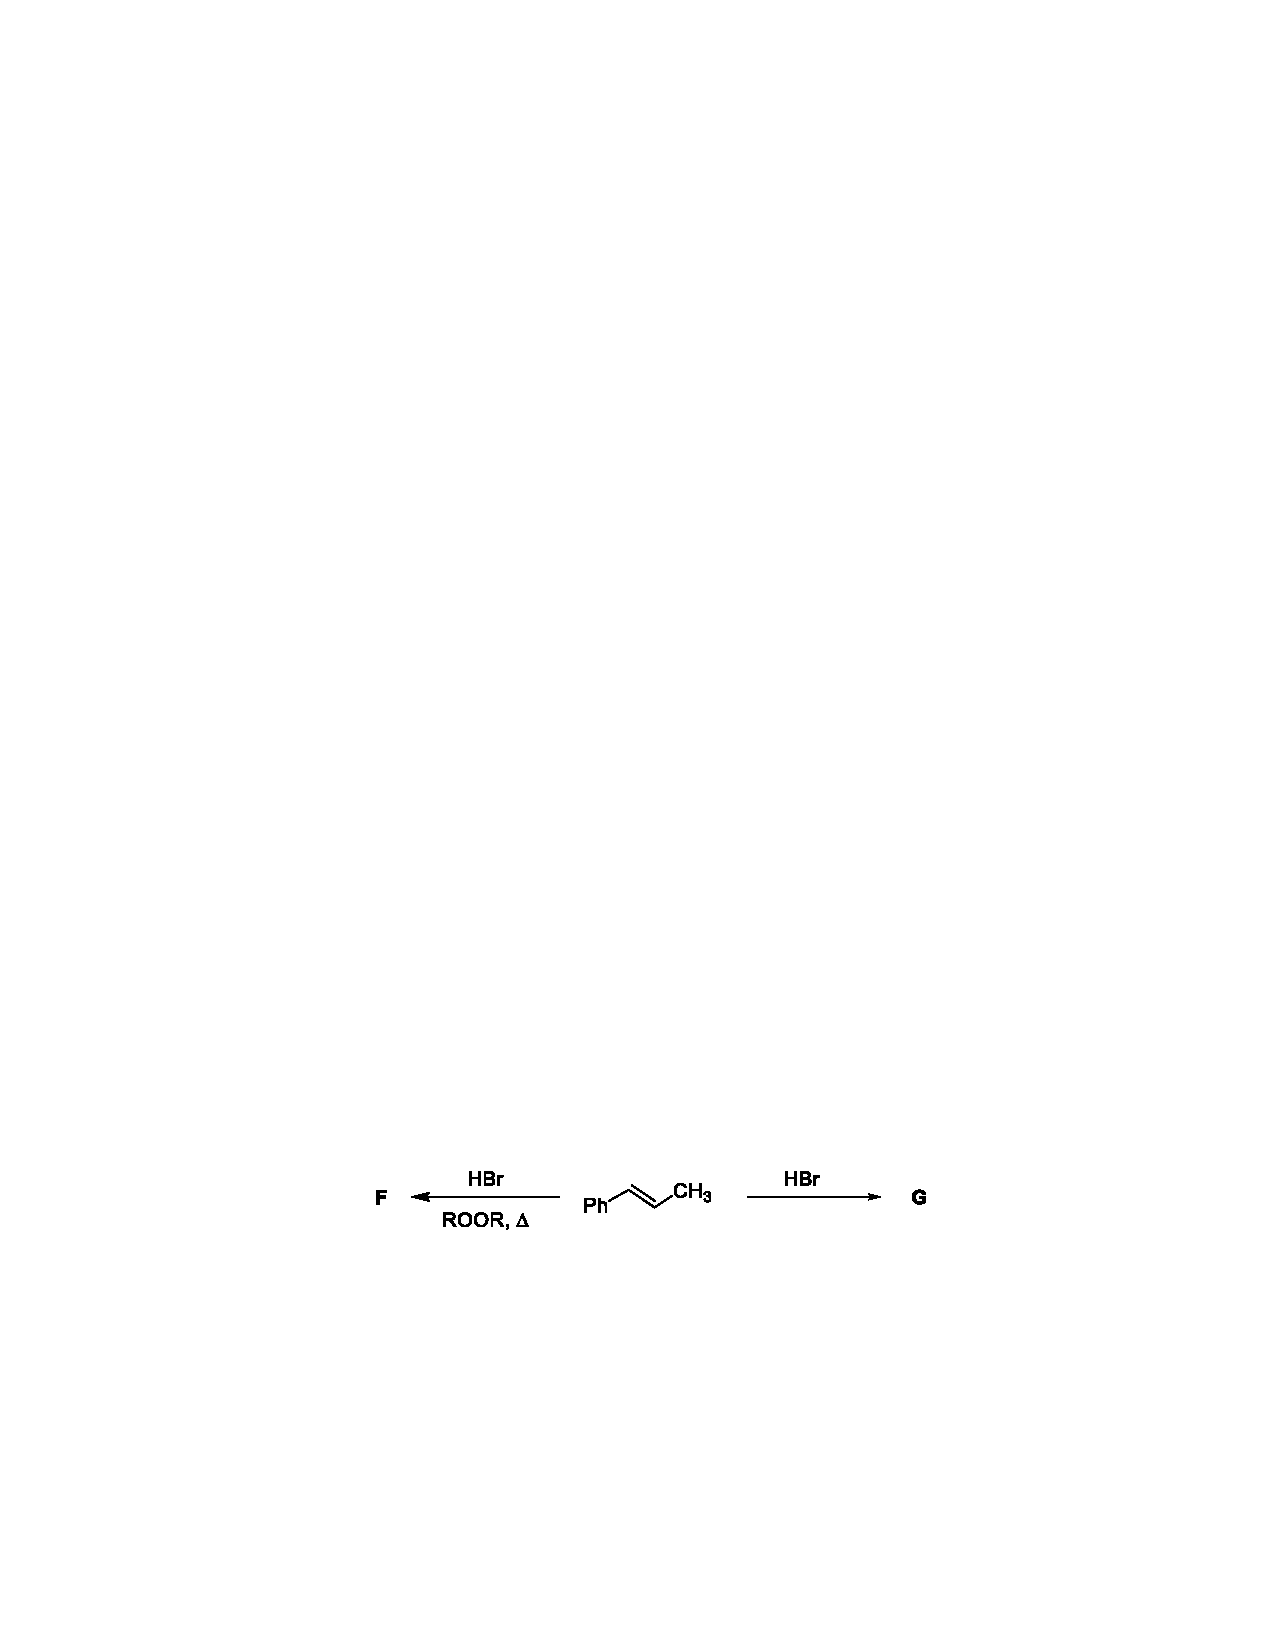
\includegraphics[width=10cm]{./pic/t4-3.pdf}
\end{figure}

\paragraph{瓦格纳-梅尔外因重排反应(Wagner-Meerwein Rearrangement,WMR)}

瓦格纳是与布特列洛夫和马尔科夫尼科夫一同在喀山大学工作的另一位著名科学家。瓦格纳认为冰片基氯(2-氯-1,7,7-三甲基双环{[}2.2.1{]}庚烷)通过一个分子内的重排反应生成了蒎烯。梅尔外因随后推广了这类反应。因此,这类反应便被称作瓦格纳-梅尔外因重排反应。这类反应会在有碳正离子中间体生成时发生。一般来说,一个碳正离子会重排为一个更稳定的碳正离子,如果可能的话还会经过邻基参与的过程。此外,如果一个反应不经历碳正离子或类似中间体的历程,重排反应便不会发生。

\begin{figure}[h!]
	\centering
	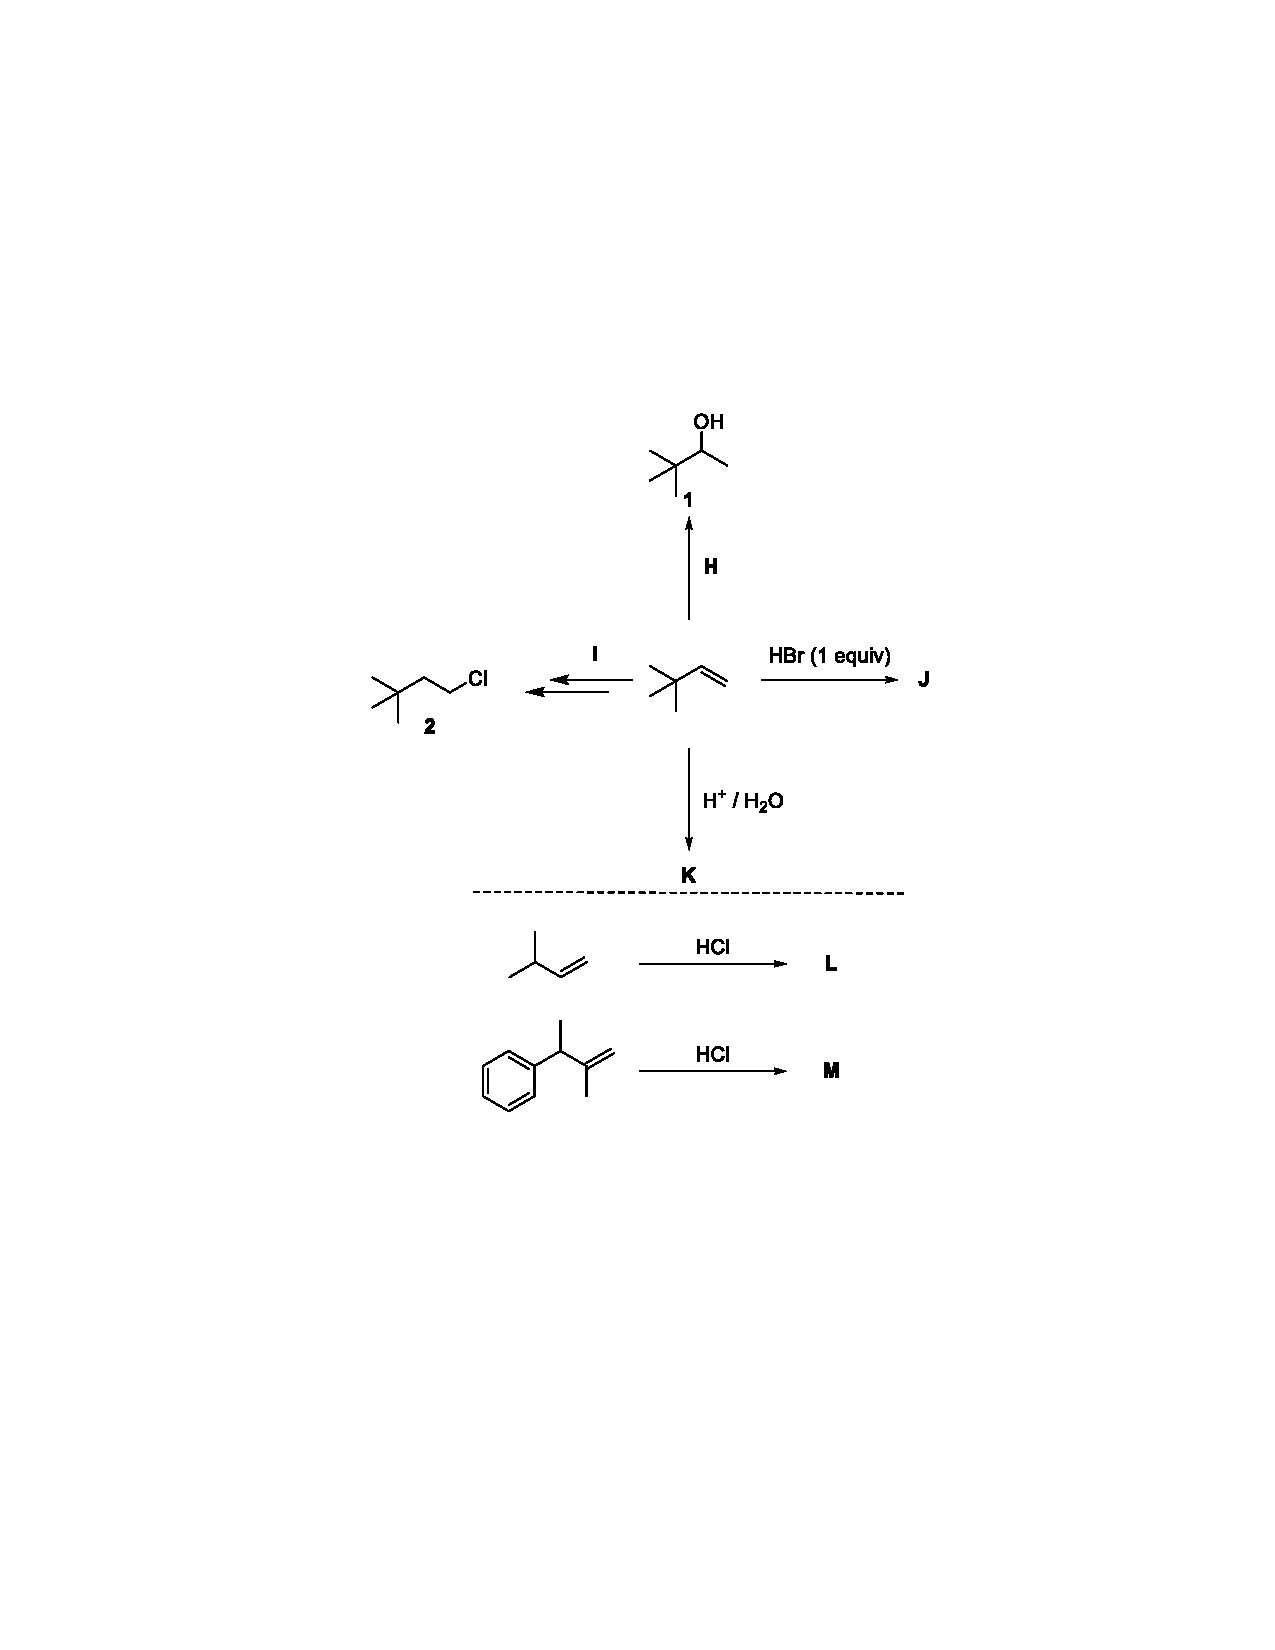
\includegraphics[width=10cm]{./pic/t4-4.pdf}
\end{figure}

\noindent\textbf{4.3.}
充分考虑每个反应过程中生成的中间体,画出试剂\textbf{H}和\textbf{I,}以及主要产物\textbf{J-M}的结构。

\paragraph{酸催化的瓦格纳-梅尔外因重排}

4,4-二甲基环己-2,5-二烯-1-酮在酸催化下反应生成化合物\textbf{N}。其NMR谱图如下所示。

\begin{figure}[h!]
	\centering
	
\includegraphics[width=7cm]{./pic/t4-5.pdf}
\end{figure}

For \textbf{N}; \textsuperscript{1}H NMR (300 MHz, CDCl\textsubscript{3}): $\delta$ = 6.95 (d,
\emph{J} = 8.0 Hz, 1H), 6.61 (d, \emph{J} = 2.8 Hz, 1H), 6.57(dd, \emph{J} = 8.0, 2.8 Hz, 1H), 5.39 (bs, 1H), 2.16 (s, 3H), 2.14 (s,
3H). \textsuperscript{13}C NMR (100 MHz, CDCl\textsubscript{3}):$\delta$ 153.4, 137.9, 130.4, 128.6, 116.6, 112.3, 19.8, 18.7.

\noindent\textbf{4.4.} 推断化合物\textbf{N}的结构并推测合理的机理。

\noindent\textbf{4.5.} 推测当一滴D\textsubscript{2}O加入NMR管的溶剂中后在
\textsuperscript{1}H NMR谱中会出现什么变化?

\paragraph{扎伊采夫规则(Zaitsev's Rule)}

扎伊采夫是化学家布特列洛夫的另一个博士生,并且也提出了一个由他的名字命名的规则------扎伊采夫规则(Zaitsev's or Saytzeff's or Saytzev's rule)。扎伊采夫规则是一个用以预测烯烃消除反应生成的优势产物的经验规则。在喀山大学,扎伊采夫研究了大量的消除反应,观测并总结了烯烃消除反应选择性的一般规律。更一般地说,扎伊采夫规则指出,在消除反应中优先生成最多取代的烯烃产物。接下来的问题主要与扎伊采夫规则有关。

\noindent\textbf{4.6.}
画出消除产物\textbf{O-Q}以及化合物\textbf{R}的结构。将\textbf{R}加热后生成的主要产物是什么?

\begin{figure}[h]
	\centering
	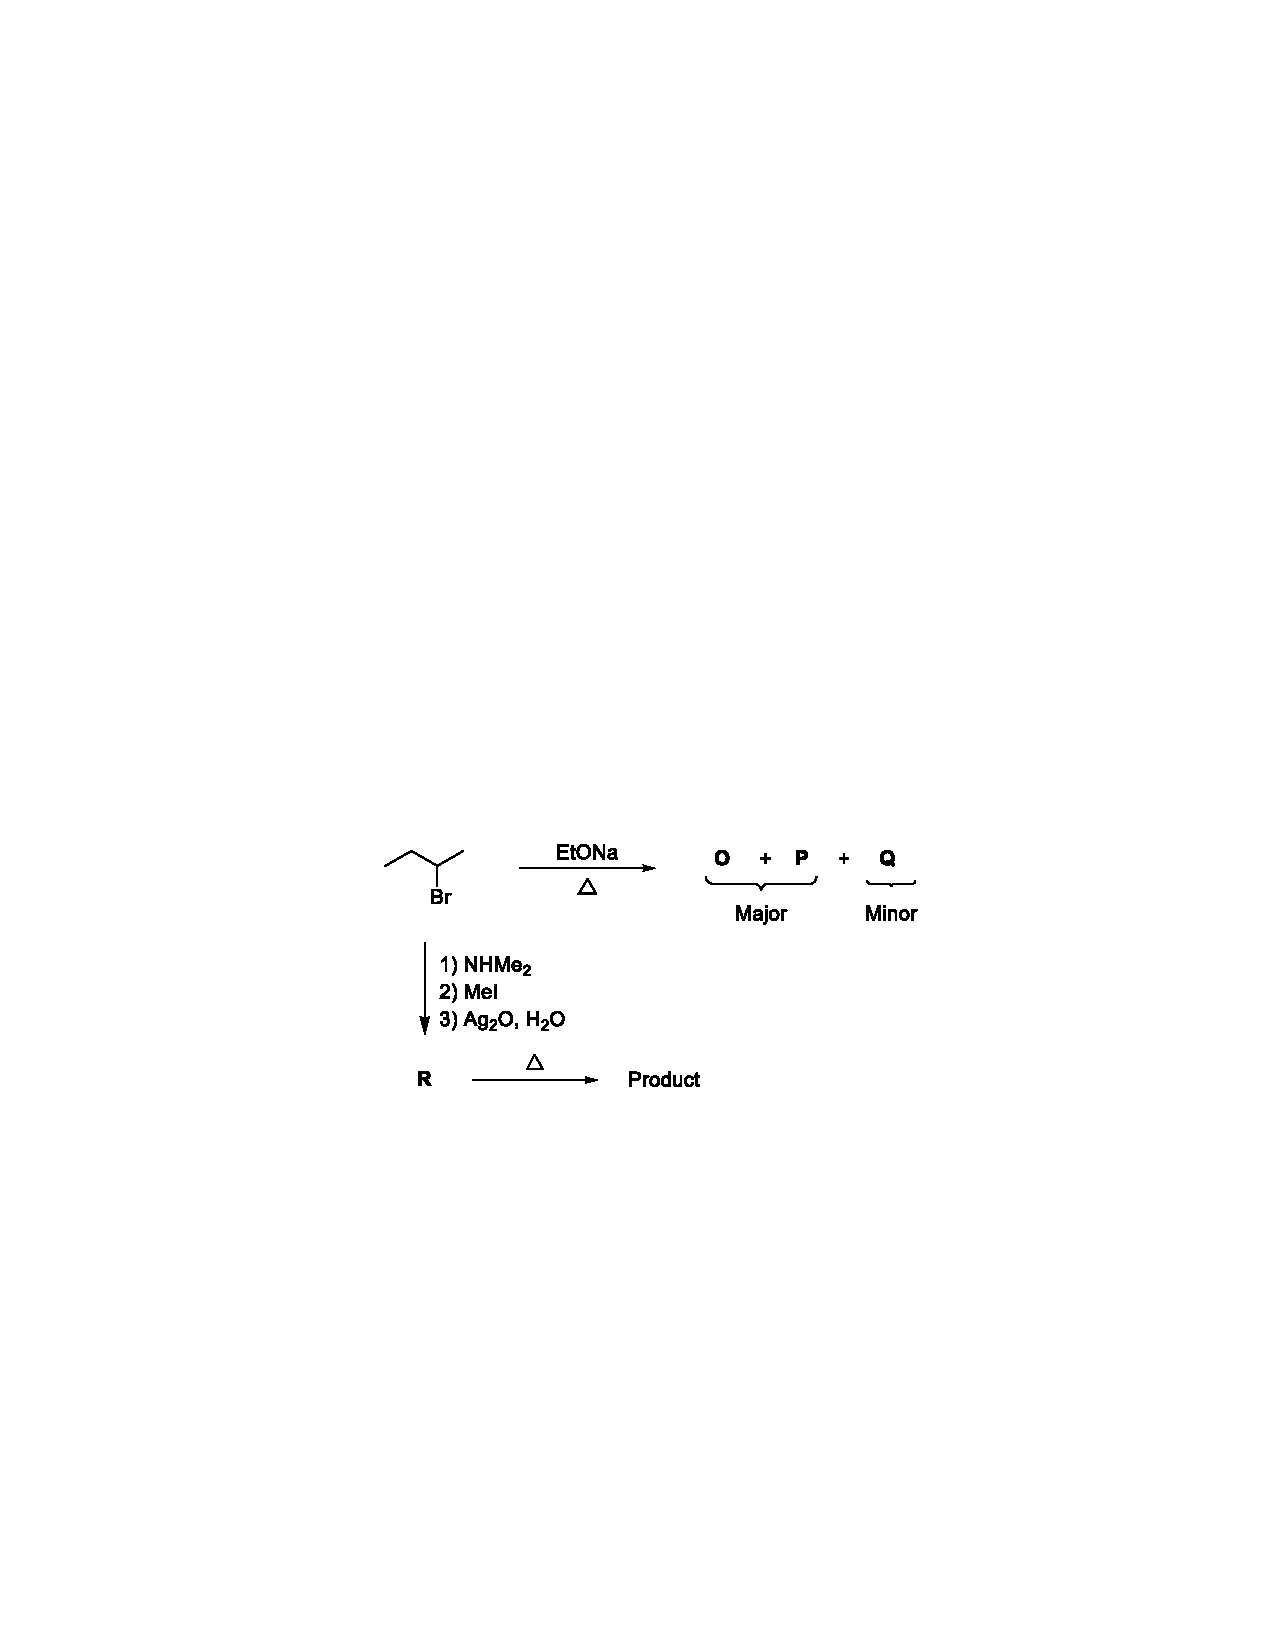
\includegraphics[width=10cm]{./pic/t4-6.pdf}
\end{figure}

\noindent\textbf{4.7.}
与EtONa相比,下列碱中哪个或哪些可以增加生成产物\textbf{Q}的比例?

\renewcommand{\labelitemi}{$\square$}
\begin{itemize}
	\item NaOMe
	\item KOMe
	\item \emph{i-}PrOK
	\item \emph{t-}BuOK
	\item NH\textsubscript{3}
	\item DBU
	\item \emph{i-}Pr\textsubscript{2}NEt
\end{itemize}
\renewcommand{\labelitemi}{$\bullet$}

\begin{figure}[h!]
	\centering
	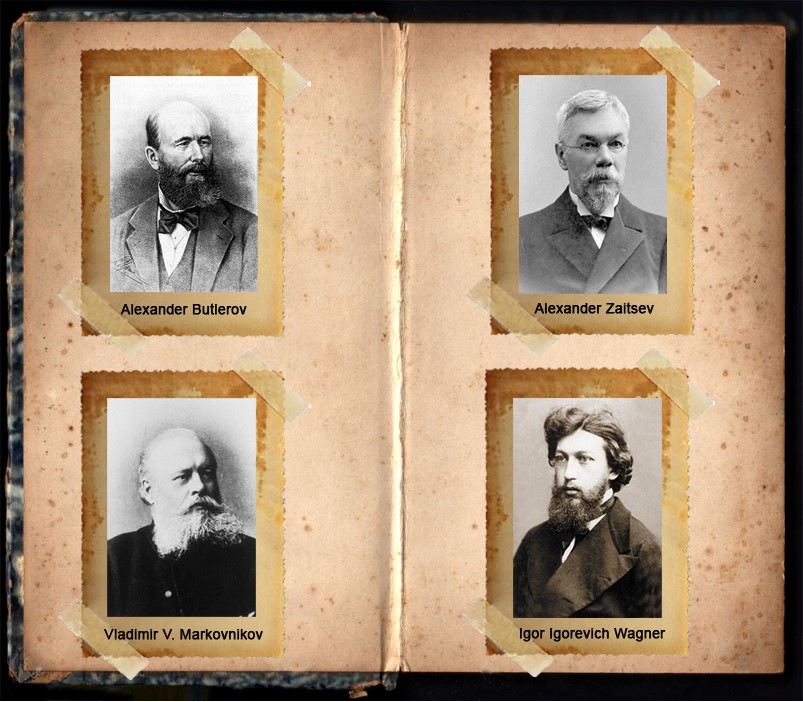
\includegraphics[width=12cm]{./pic/t4-1.jpg}
\end{figure}
